\begin{frame}
	\frametitle{O problema}
	\begin{figure}[h]
		\caption{Óbitos no trânsito de 2004 a 2015}
		\centering
		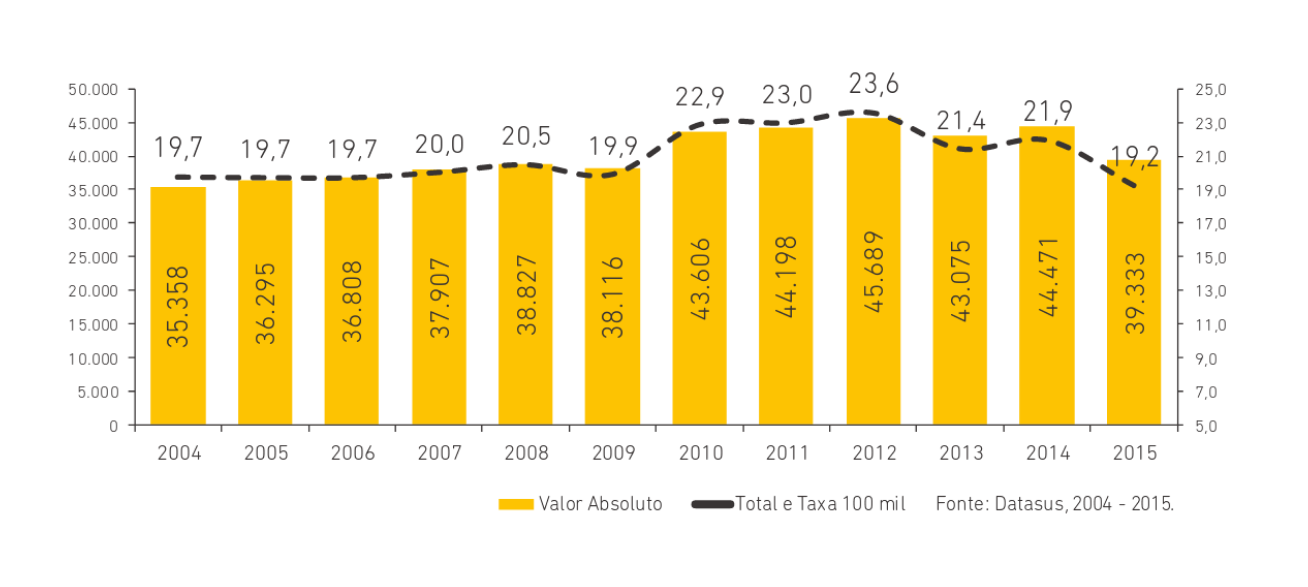
\includegraphics[width=1\textwidth]{imagens/obto}
	\end{figure}
\end{frame}

\begin{frame}
	\frametitle{O problema \textit{continuação}}
	\begin{figure}[h]
		\caption{Vítimas não fatais no trânsito de 2004 a 2015}
		\centering
		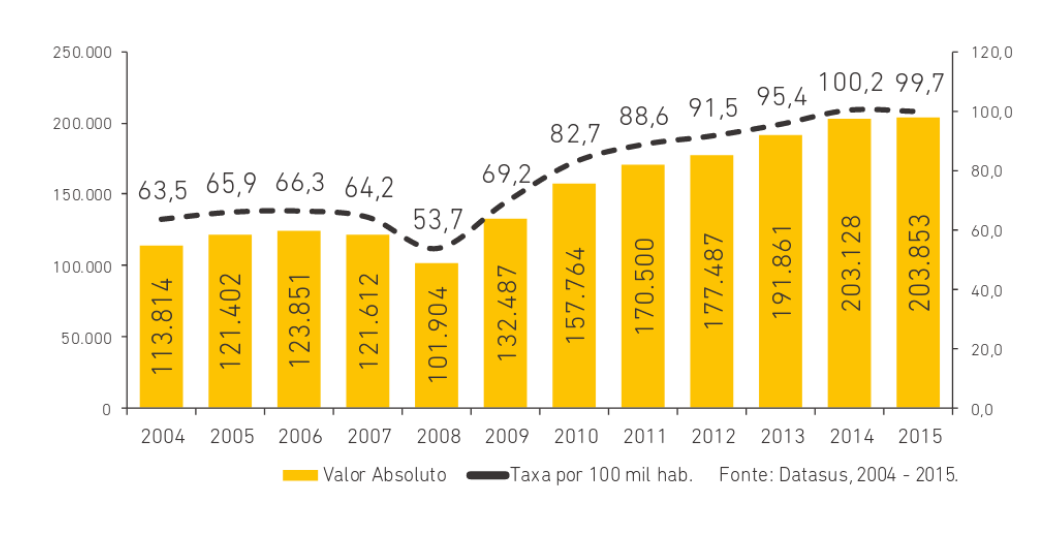
\includegraphics[width=1\textwidth]{imagens/ferido}
	\end{figure}
\end{frame}

\begin{frame}
	\frametitle{Efeitos do problema}
	\begin{columns}
		\begin{column}{0.5\textwidth}
			\begin{figure}[h]
				\caption{10 maiores causas de morte em 2015}
				\centering
				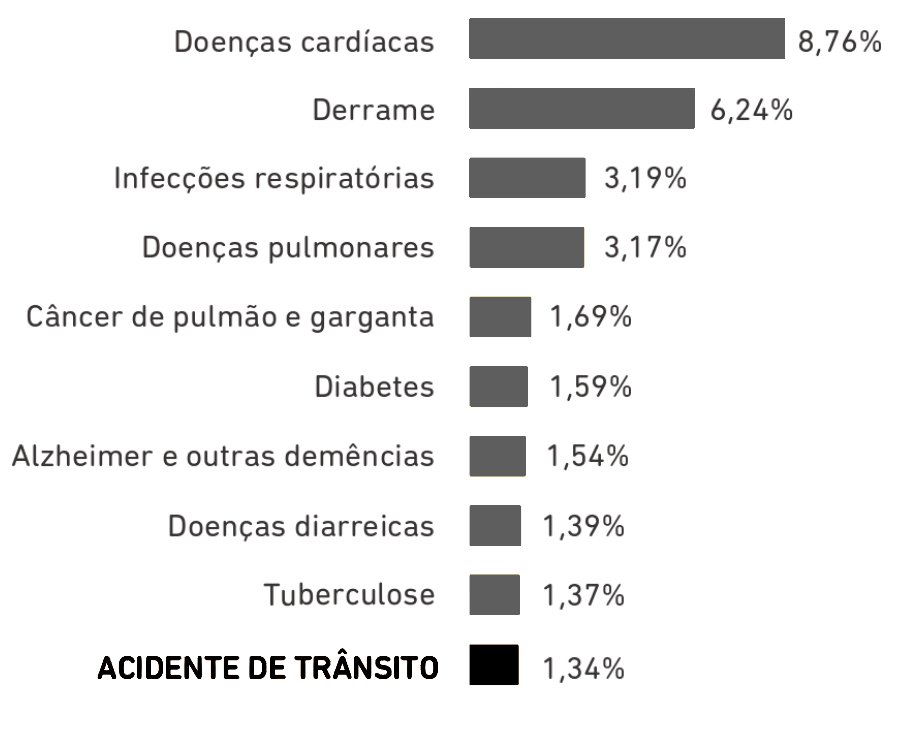
\includegraphics[width=1\textwidth]{imagens/acidente-transito}
			\end{figure}
		\end{column}
		\begin{column}{0.5\textwidth} 
			Para o Brasil isso representou R\$ 19 Bilhões\cite{ambev}.
		\end{column}
	\end{columns}	
\end{frame}